\documentclass{article}
\usepackage{graphicx}
\usepackage[rightcaption]{sidecap}
\graphicspath{ {./billeder/} }
\usepackage{amsmath,amsfonts,stmaryrd,amssymb}
\usepackage[ruled]{algorithm2e}
\usepackage[framemethod=tikz]{mdframed}
\usepackage{parskip}
\usepackage{nameref}
\usepackage{booktabs}
\usepackage{tabularx}
\usepackage{geometry}
\geometry{
	paper=a4paper,
	top=2.5cm,
	bottom=3cm,
	left=2.5cm,
	right=2.5cm,
	headheight=14pt,
	footskip=1.5cm,
	headsep=1.2cm,
	%showframe, % Uncomment to show how the type block is set on the page
}

\usepackage[utf8]{inputenc}
\usepackage[T1]{fontenc}
\usepackage{XCharter}
\usepackage{graphicx}

\author {Jesper Toplund}
\title{Roadmap for komponenter}
\date{}

\begin{document}
\maketitle

\vspace{20 mm}
\begin{quote}
    \textit{}
\end{quote}
\newpage{}
\clearpage

\section{Baggrund}
\subsection{Formål}

% \subsection{Datagrundlag}
% Denne sektion kan udelades.

\subsection{Omfang}

\section{Analyse af komponenter}

\subsection{Akamai}
\begin{figure}[h]
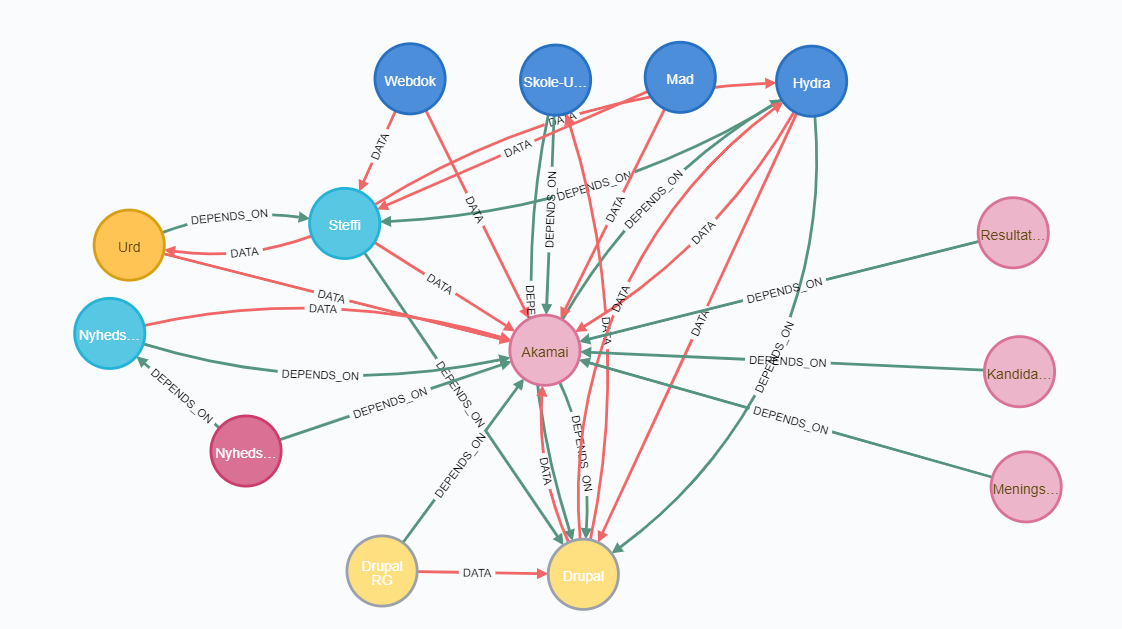
\includegraphics[width=300pt]{Akamai.PNG}
\caption{MATCH (x\{name:'Akamai'\})- -(y) RETURN x,y}
\end{figure}
\subsubsection{Kort beskrivelse}
Akamai benyttes som det primære CDN (content delivery Network). 
Det er dermed ikke et produkt som er udviklet hverken af eller for DR, 
men et produkt som vi er afhængige af. 
\subsubsection{Anbefalet handling}
Akamai som CDN udfylder fint de behov som DR har. 

Vi kan med fordel kikke på om vi benytter fornuftige cache timeouts eller om vores hjemmeside er struktureret til at få mest muligt ud af CDN.
\subsubsection{Overslag}
Indgår ikke som sådan i roadmap.



\subsection{Hydra}
\begin{figure}[h]
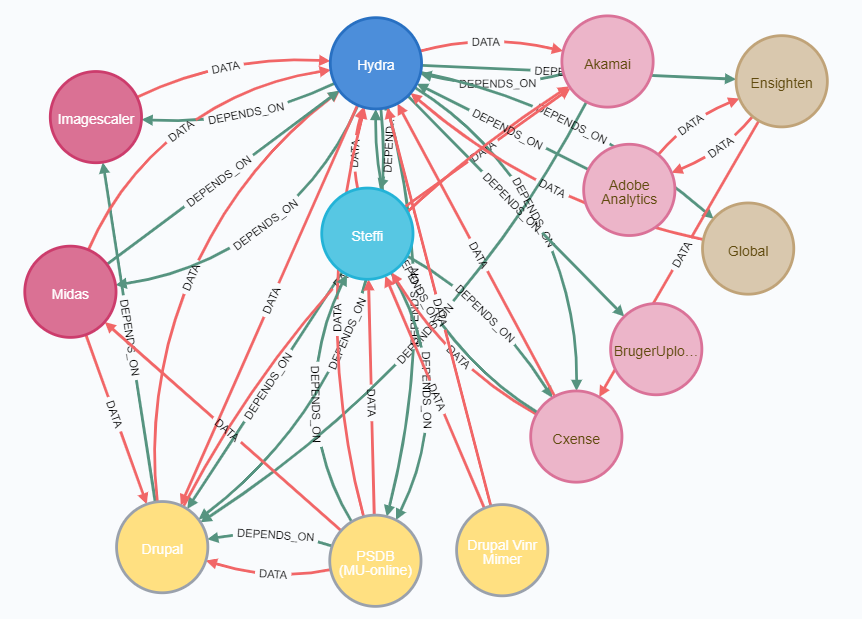
\includegraphics[width=300pt]{Hydra.PNG}
\caption{MATCH (x\{name:'Hydra'\})- -(y) RETURN x,y}
\end{figure}
\subsubsection{Kort beskrivelse}
Web-frontend, der varetager indholdsvisning for artikler og forsider. Anvender Drupal-visning til sider, der endnu ikke understøttes af Hydra.
Ovenstående figur viser at der er et højt antal afhængigheder til mange systemer. Det skal undersøges nærmere om de alle er aktuelle.
\subsubsection{Anbefalet handling}
Hydra er beskrevet som at den direkte henter data fra og sender data til Drupal. Er det korrekt, så springer den flere lag over i referencearkitekturen.
Hydra burde kun afhænge af platform utilities, platform services, product services eller content aggregation.
% TODO Verificer at alle de beskrevne afhængigheder også er aktuelle afhængigheder.
\subsubsection{Overslag}
Afklaring nødvendigt før det kan estimeres.


\subsection{Steffi}
\begin{figure}[h]
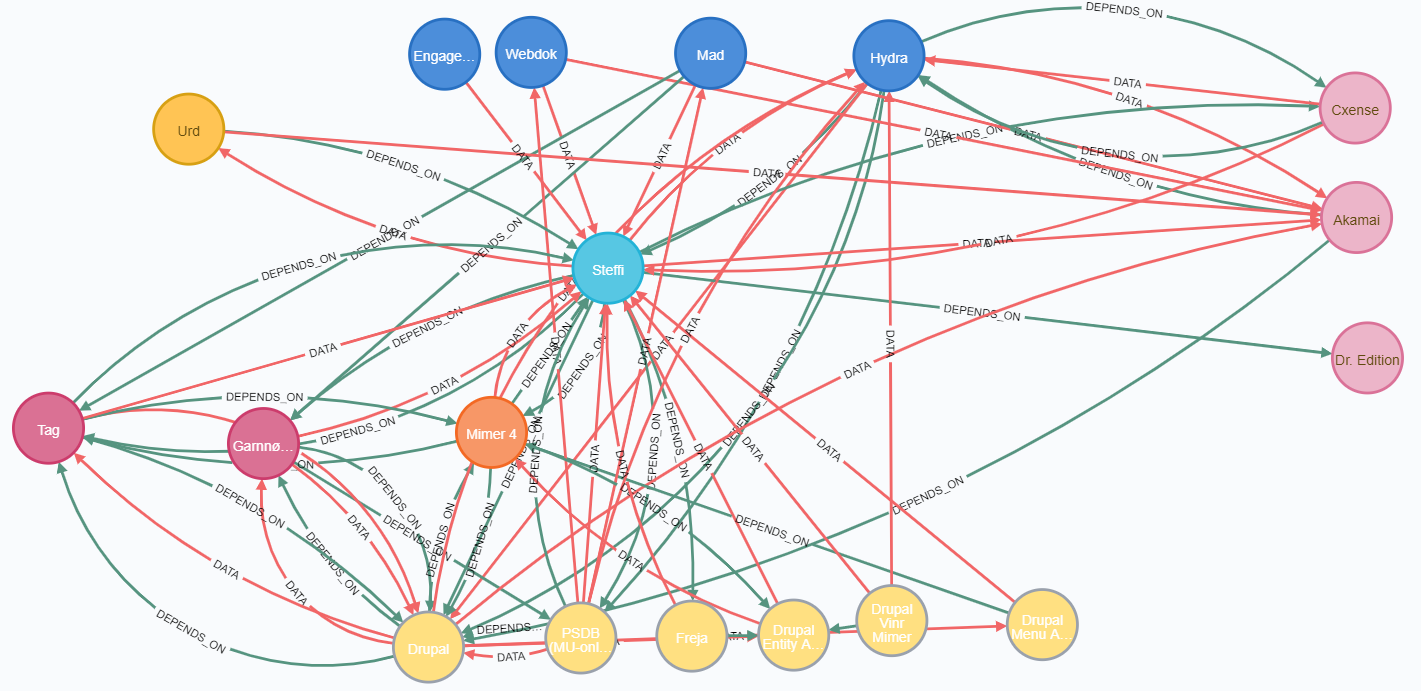
\includegraphics[width=300pt]{Steffi.PNG}
\caption{MATCH (x\{name:'Steffi'\})- -(y) RETURN x,y}
\end{figure}
\subsubsection{Kort beskrivelse}
Forespørgselslag, der tilbyder GraphQL-grænseflader til frontendapplikationer.
benyttes Content aggregering.
\subsubsection{Anbefalet handling}
\subsubsection{Overslag}


\subsection{Talentholdet}
\begin{figure}[h]
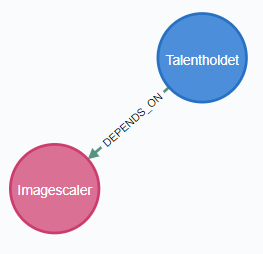
\includegraphics[width=300pt]{Talentholdet.PNG}
\caption{MATCH (x\{name:'Talentholdet'\})- -(y) RETURN x,y}
\end{figure}
\subsubsection{Kort beskrivelse}
Talentholdet er en rekrutteringsplatform for nye talenter til DR. Talentholdet har sin egen database hvori den gemmer personidentificerbar data i krypteret form. Talentholdet afhænger af Imagescaler
\subsubsection{Anbefalet handling}
Talentholdet udfører en mindre opgave som det er muligt at diskutere værdien af. Vi bør få afklaret med forretningen om vi eventuelt kan pensionere programmet. Der er en del kodegæld i programmet og GDPR sletninger er en manuel process.
Prioriteten af Talentholdet er dog ret lav, så den manuelle process kan tolereres.
\subsubsection{Overslag}
N/A

\subsection{Elements}
\begin{figure}[h]
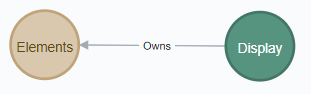
\includegraphics[width=200pt]{Elements.PNG}
\caption{MATCH (x\{name:'Elements'\})- -(y) RETURN x,y}
\end{figure}
\subsubsection{Kort beskrivelse}
Elements er DR's centrale komponentbibliotek, som består af FE komponenter. Elements er kodet i React. Elements benyttes af en række af vores Frontend products.
\subsubsection{Anbefalet handling}
Elements benyttes en række af vores Frontend products og passer fint ind i vores reference arkitektur
\subsubsection{Overslag}
N/A

\subsection{Webdok}
\begin{figure}[h]
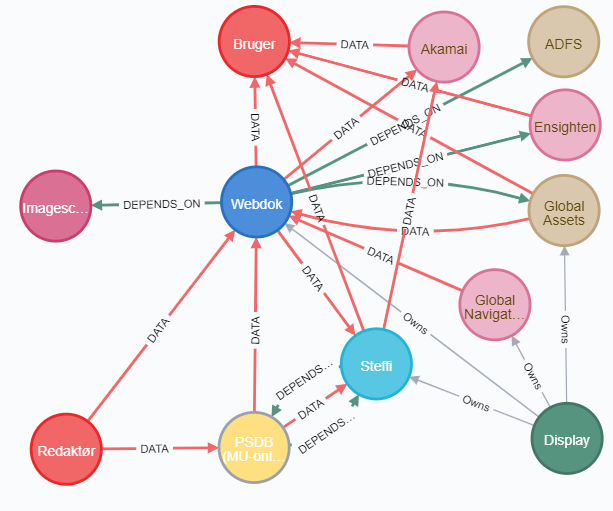
\includegraphics[width=300pt]{Webdok.PNG}
\caption{MATCH (x\{name:'Webdok'\})- -(y) RETURN x,y}
\end{figure}
\subsubsection{Kort beskrivelse}
CMS og præsentation af featureartikler i særformater.	
Præsentationslag (Node.js) trækker data fra API (.NET). Redaktørgrænseflade er bygget ind i præsentationslaget.
\subsubsection{Anbefalet handling}
Hvordan Webdok er flettet ind i vores nuværende arkitektur skal undersøges nærmere. Dokumentationen som den står nu giver et lidt mudret billede
% TODO
\subsubsection{Overslag}
Ukendt.
\newpage{}
\clearpage


\subsection{Skole-Undervisning}
\begin{figure}[h]
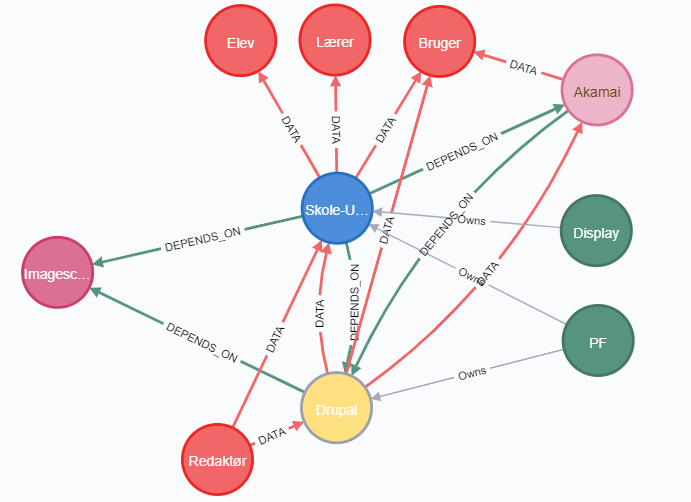
\includegraphics[width=300pt]{Skole-Undervisning.PNG}
\caption{MATCH (x\{name:'Skole-Undervisning'\})- -(y) RETURN x,y}
\end{figure}
\subsubsection{Kort beskrivelse}
Skole og Undervisning er et site, der formidler undervisningsforløb og undervisningsmateriale til Skoler.  Sitet er opbygget i Drupal, men har en række specialløsninger konstrueret for at kunne samle temaer og autogenerere faktabokse etc. 
\subsubsection{Anbefalet handling}
Skole-Undervisning passer ikke ind i referencearkitekturen, idet den udgør sin helt egen silo og udstiller data direkte til slutbrugere via Akamai. 
Afhængigt af levetiden for projektet (gartner Time model) skal vi overveje hvad vi gør ved projektet.
\subsubsection{Overslag}
Afklaring mangler.
%TODO

\subsection{Mad}
\begin{figure}[h]
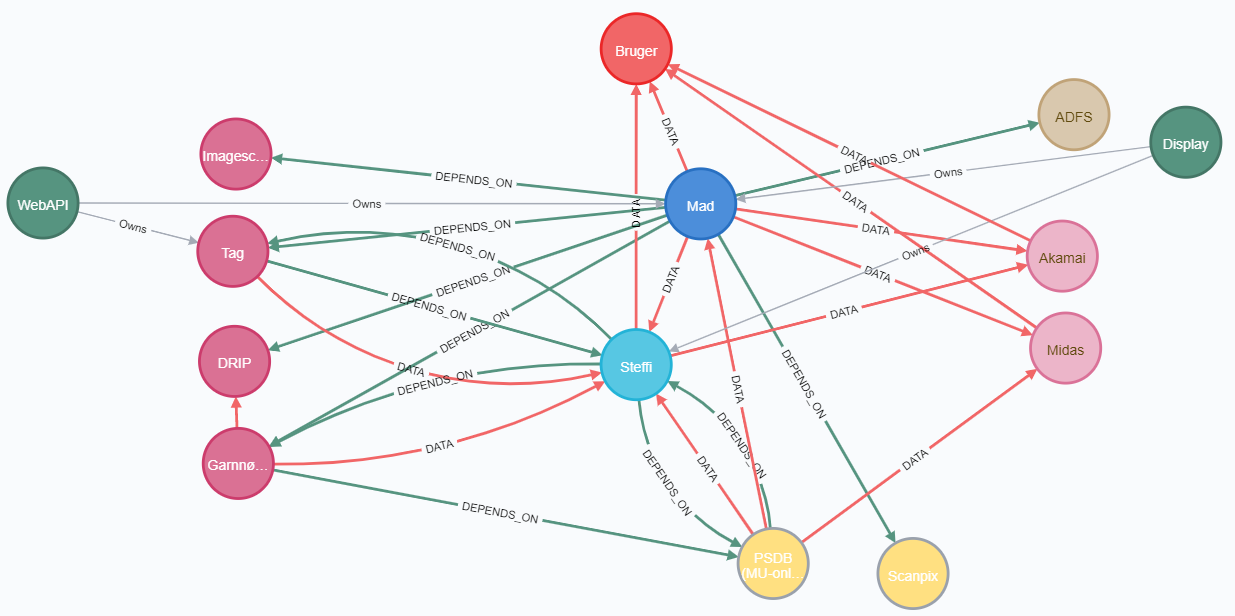
\includegraphics[width=300pt]{Mad.PNG}
\caption{MATCH (x\{name:'Mad'\})- -(y) RETURN x,y}
\end{figure}
\subsubsection{Kort beskrivelse}
Mad er en applikation, der håndterer opskrifter, artikler og opskriftssamlinger. Mad er bygget som Headless Drupal med egen RG til opskrifter. Artikler publiceres gennem Drupal. 
\subsubsection{Anbefalet handling}
Mad passer ikke helt ind i referencearkitekturen som beskrevet. Om det er en mangel i dokumentationen eller i arkitekturen skal undersøges. (hvorfor tilgår Steffi Mad direkte og ikke igennem f.eks. Mimer?)
\subsubsection{Overslag}
Afklaring mangler
%TODO

\subsection{Nyhedsapp-Frontend}
\begin{figure}[h]
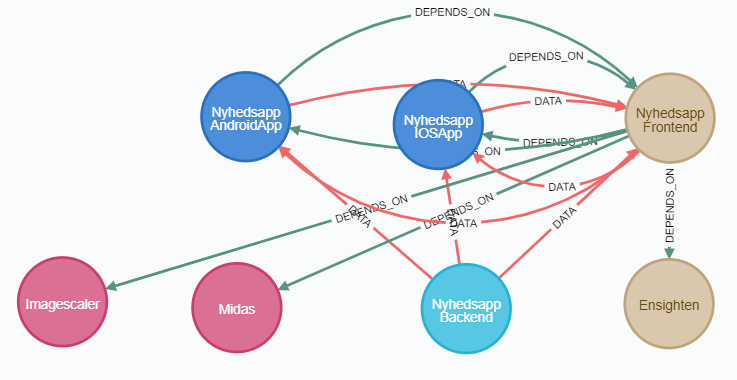
\includegraphics[width=300pt]{Nyhedsapp-Frontend.PNG}
\caption{MATCH (x\{name:'Nyhedsapp Frontend'\})- -(y) RETURN x,y}
\end{figure}
\subsubsection{Kort beskrivelse}
Præsentationslag for indhold i Nyhedsapp, således at visningen mellem iOS og Android er homogen, samt har lignende homogenitet til visningen på DR.dk
Nyhedsapp-Frontend er ikke en selvstændig applikation, men et delt kodelag der anvendes af IOS og Android udgaven af nyhedsappen. 
\subsubsection{Anbefalet handling}
Nyhedsapp-Frontend vurderes ikke selvstændigt i forhold til referencearkitekturen.
\subsubsection{Overslag}
N/A

\subsection{Nyhedsapp IOS}
\begin{figure}[h]
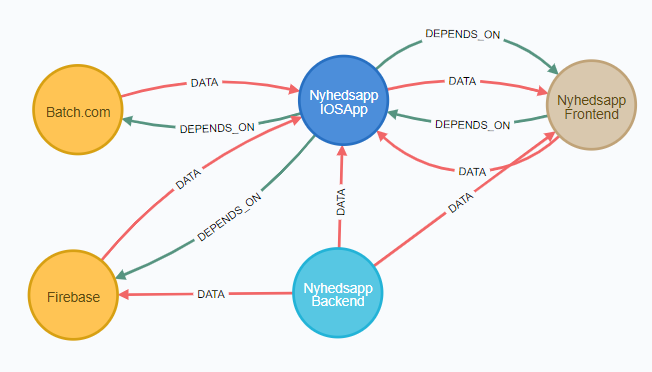
\includegraphics[width=300pt]{Nyhedsapp-IOS.PNG}
\caption{MATCH (x\{name:'Nyhedsapp IOSApp'\})- -(y) RETURN x,y}
\end{figure}
\subsubsection{Kort beskrivelse}
Afvikler Nyhedsapp Frontend, integrerer til iOS-native funktionalitet
\subsubsection{Anbefalet handling}
Nyhedsapp til både IOS og Android overholder referencearkitekturen. Der er måske ønsker om at opdatere applikationerne så de får et mere moderne udtryk på telefonerne. Dette ønske er dog et forretningsdrevet ønske og ikke en nødvendighed set ud fra reference arkitekturen
\subsubsection{Overslag}
Ingen ændringer nødvendige

\subsection{Nyhedsapp AndroidApp}
\begin{figure}[h]
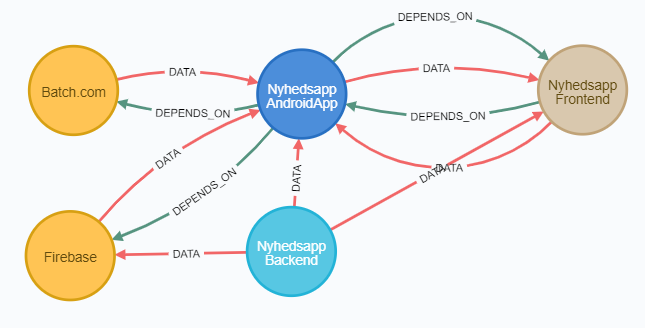
\includegraphics[width=300pt]{Nyhedsapp-Android.PNG}
\caption{MATCH (x\{name:'Nyhedsapp AndroidApp'\})- -(y) RETURN x,y}
\end{figure}
\subsubsection{Kort beskrivelse}
Native Android-wrapper, der afvikler Nyhedsapp Frontend
\subsubsection{Anbefalet handling}
Nyhedsapp til både IOS og Android overholder referencearkitekturen. Der er måske ønsker om at opdatere applikationerne så de får et mere moderne udtryk på telefonerne. Dette ønske er dog et forretningsdrevet ønske og ikke en nødvendighed set ud fra reference arkitekturen
\subsubsection{Overslag}
Ingen ændringer nødvendige



\subsection{Batch.com}
\begin{figure}[h]
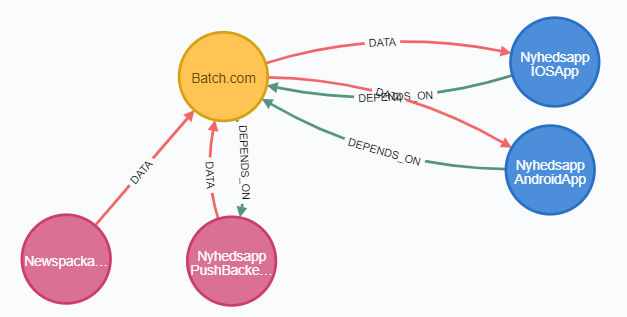
\includegraphics[width=300pt]{Batch-com.PNG}
\caption{MATCH (x\{name:'Batch.com'\})- -(y) RETURN x,y}
\end{figure}
\subsubsection{Kort beskrivelse}
SaaS tejneste der benyttes til push af beskeder til NyhedsApp
Distribuerer data til Nyhedsapp-instanser, med mulighed for dublikeringskontrol så den samme enhed kun modtager data én gang, og ligeledes en opfølgningsmulighed så devices der var utilgængelige på udsendelsestidspunktet, opdateres når de er tilgængelige igen
\subsubsection{Anbefalet handling}
Tjenesten passer ind i vores referencearkitektur. Om Batch.com bliver ved med at være den bedste løsning for push af beskeder vil vi ikke tage stilling til i dette dokument.
\subsubsection{Overslag}
Ingen ændringer nødvendige


\subsection{Firebase}
\begin{figure}[h]
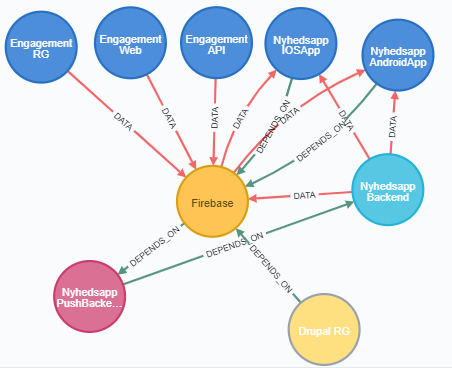
\includegraphics[width=300pt]{Firebase.PNG}
\caption{MATCH (x\{name:'Firebase'\})- -(y) RETURN x,y}
\end{figure}
\subsubsection{Kort beskrivelse}
SaaS tjeneste der benyttes til Pusg service af flere applikationer:
Nyhedsapp, Drupal RG ("hvem er inde på min artikel")
\subsubsection{Anbefalet handling}
Tjenesten passer ind i vores referencearkitektur. Om Firebase bliver ved med at være den bedste løsning for push af beskeder vil vi ikke tage stilling til i dette dokument.
\subsubsection{Overslag}
\subsection{OCS}


\begin{figure}[h]

\includegraphics[width=300pt]{CHANGE.PNG}
\caption{MATCH (x\{name:'CHANGE'\})- -(y) RETURN x,y}
\end{figure}
\subsubsection{Kort beskrivelse}
\subsubsection{Anbefalet handling}
\subsubsection{Overslag}
\subsection{Garnnøgle}


\begin{figure}[h]

\includegraphics[width=300pt]{CHANGE.PNG}
\caption{MATCH (x\{name:'CHANGE'\})- -(y) RETURN x,y}
\end{figure}
\subsubsection{Kort beskrivelse}
\subsubsection{Anbefalet handling}
\subsubsection{Overslag}


\subsection{Drupal}
\begin{figure}[h]

\includegraphics[width=300pt]{CHANGE.PNG}
\caption{MATCH (x\{name:'CHANGE'\})- -(y) RETURN x,y}
\end{figure}
\subsubsection{Kort beskrivelse}
\subsubsection{Anbefalet handling}
\subsubsection{Overslag}
\subsection{Mimer 1.0 API}
\begin{figure}[h]

\includegraphics[width=300pt]{CHANGE.PNG}
\caption{MATCH (x\{name:'CHANGE'\})- -(y) RETURN x,y}
\end{figure}
\subsubsection{Kort beskrivelse}
\subsubsection{Anbefalet handling}
\subsubsection{Overslag}
\subsection{Drupal RG}
\begin{figure}[h]

\includegraphics[width=300pt]{CHANGE.PNG}
\caption{MATCH (x\{name:'CHANGE'\})- -(y) RETURN x,y}
\end{figure}
\subsubsection{Kort beskrivelse}
\subsubsection{Anbefalet handling}
\subsubsection{Overslag}
\subsection{Drupal Entity API}
\begin{figure}[h]

\includegraphics[width=300pt]{CHANGE.PNG}
\caption{MATCH (x\{name:'CHANGE'\})- -(y) RETURN x,y}
\end{figure}
\subsubsection{Kort beskrivelse}
\subsubsection{Anbefalet handling}
\subsubsection{Overslag}
\newpage{}
\clearpage
\subsection{Drupal Menu API}
\begin{figure}[h]

\includegraphics[width=300pt]{CHANGE.PNG}
\caption{MATCH (x\{name:'CHANGE'\})- -(y) RETURN x,y}
\end{figure}
\subsubsection{Kort beskrivelse}
\subsubsection{Anbefalet handling}
\subsubsection{Overslag}
\subsection{Ensighten}
\begin{figure}[h]

\includegraphics[width=300pt]{CHANGE.PNG}
\caption{MATCH (x\{name:'CHANGE'\})- -(y) RETURN x,y}
\end{figure}
\subsubsection{Kort beskrivelse}
\subsubsection{Anbefalet handling}
\subsubsection{Overslag}
\subsection{Ad Server}
\begin{figure}[h]

\includegraphics[width=300pt]{CHANGE.PNG}
\caption{MATCH (x\{name:'CHANGE'\})- -(y) RETURN x,y}
\end{figure}
\subsubsection{Kort beskrivelse}
\subsubsection{Anbefalet handling}
\subsubsection{Overslag}
\subsection{Midas}
\begin{figure}[h]

\includegraphics[width=300pt]{CHANGE.PNG}
\caption{MATCH (x\{name:'CHANGE'\})- -(y) RETURN x,y}
\end{figure}
\subsubsection{Kort beskrivelse}
\subsubsection{Anbefalet handling}
\subsubsection{Overslag}
\subsection{PSDB (MU-online)}
\begin{figure}[h]

\includegraphics[width=300pt]{CHANGE.PNG}
\caption{MATCH (x\{name:'CHANGE'\})- -(y) RETURN x,y}
\end{figure}
\subsubsection{Kort beskrivelse}
\subsubsection{Anbefalet handling}
\subsubsection{Overslag}
\subsection{Scanpix}
\begin{figure}[h]

\includegraphics[width=300pt]{CHANGE.PNG}
\caption{MATCH (x\{name:'CHANGE'\})- -(y) RETURN x,y}
\end{figure}
\subsubsection{Kort beskrivelse}
\subsubsection{Anbefalet handling}
\subsubsection{Overslag}
\subsection{Cxense}
\begin{figure}[h]

\includegraphics[width=300pt]{CHANGE.PNG}
\caption{MATCH (x\{name:'CHANGE'\})- -(y) RETURN x,y}
\end{figure}
\subsubsection{Kort beskrivelse}
\subsubsection{Anbefalet handling}
\subsubsection{Overslag}
\subsection{Adobe Analytics}
\begin{figure}[h]

\includegraphics[width=300pt]{CHANGE.PNG}
\caption{MATCH (x\{name:'CHANGE'\})- -(y) RETURN x,y}
\end{figure}
\subsubsection{Kort beskrivelse}
\subsubsection{Anbefalet handling}
\subsubsection{Overslag}
\subsection{Pressebilleder}
\begin{figure}[h]

\includegraphics[width=300pt]{CHANGE.PNG}
\caption{MATCH (x\{name:'CHANGE'\})- -(y) RETURN x,y}
\end{figure}
\subsubsection{Kort beskrivelse}
\subsubsection{Anbefalet handling}
\subsubsection{Overslag}
\subsection{WebCMS}
\begin{figure}[h]

\includegraphics[width=300pt]{CHANGE.PNG}
\caption{MATCH (x\{name:'CHANGE'\})- -(y) RETURN x,y}
\end{figure}
\subsubsection{Kort beskrivelse}
\subsubsection{Anbefalet handling}
\subsubsection{Overslag}
\subsection{DR Search}
\begin{figure}[h]

\includegraphics[width=300pt]{CHANGE.PNG}
\caption{MATCH (x\{name:'CHANGE'\})- -(y) RETURN x,y}
\end{figure}
\subsubsection{Kort beskrivelse}
\subsubsection{Anbefalet handling}
\subsubsection{Overslag}
\subsection{Nyhedsbreve}
\begin{figure}[h]

\includegraphics[width=300pt]{CHANGE.PNG}
\caption{MATCH (x\{name:'CHANGE'\})- -(y) RETURN x,y}
\end{figure}
\subsubsection{Kort beskrivelse}
\subsubsection{Anbefalet handling}
\subsubsection{Overslag}
\newpage{}
\clearpage
\subsection{DR Billeder}
\begin{figure}[h]

\includegraphics[width=300pt]{CHANGE.PNG}
\caption{MATCH (x\{name:'CHANGE'\})- -(y) RETURN x,y}
\end{figure}
\subsubsection{Kort beskrivelse}
\subsubsection{Anbefalet handling}
\subsubsection{Overslag}
\subsection{DR.DK oEmbed S3 bucket}
\begin{figure}[h]

\includegraphics[width=300pt]{CHANGE.PNG}
\caption{MATCH (x\{name:'CHANGE'\})- -(y) RETURN x,y}
\end{figure}
\subsubsection{Kort beskrivelse}
\subsubsection{Anbefalet handling}
\subsubsection{Overslag}
\subsection{Mimer 3}
\begin{figure}[h]

\includegraphics[width=300pt]{CHANGE.PNG}
\caption{MATCH (x\{name:'CHANGE'\})- -(y) RETURN x,y}
\end{figure}
\subsubsection{Kort beskrivelse}
\subsubsection{Anbefalet handling}
\subsubsection{Overslag}
\subsection{Mimer 4}
\begin{figure}[h]

\includegraphics[width=300pt]{CHANGE.PNG}
\caption{MATCH (x\{name:'CHANGE'\})- -(y) RETURN x,y}
\end{figure}
\subsubsection{Kort beskrivelse}
\subsubsection{Anbefalet handling}
\subsubsection{Overslag}
\subsection{Tag}
\begin{figure}[h]

\includegraphics[width=300pt]{CHANGE.PNG}
\caption{MATCH (x\{name:'CHANGE'\})- -(y) RETURN x,y}
\end{figure}
\subsubsection{Kort beskrivelse}
\subsubsection{Anbefalet handling}
\subsubsection{Overslag}
\subsection{Urd}
\begin{figure}[h]

\includegraphics[width=300pt]{CHANGE.PNG}
\caption{MATCH (x\{name:'CHANGE'\})- -(y) RETURN x,y}
\end{figure}
\subsubsection{Kort beskrivelse}
\subsubsection{Anbefalet handling}
\subsubsection{Overslag}
\subsection{Infomedia}
\begin{figure}[h]

\includegraphics[width=300pt]{CHANGE.PNG}
\caption{MATCH (x\{name:'CHANGE'\})- -(y) RETURN x,y}
\end{figure}
\subsubsection{Kort beskrivelse}
\subsubsection{Anbefalet handling}
\subsubsection{Overslag}
\subsection{Auth0}
\begin{figure}[h]

\includegraphics[width=300pt]{CHANGE.PNG}
\caption{MATCH (x\{name:'CHANGE'\})- -(y) RETURN x,y}
\end{figure}
\subsubsection{Kort beskrivelse}
\subsubsection{Anbefalet handling}
\subsubsection{Overslag}
\subsection{Identity API}
\begin{figure}[h]

\includegraphics[width=300pt]{CHANGE.PNG}
\caption{MATCH (x\{name:'CHANGE'\})- -(y) RETURN x,y}
\end{figure}
\subsubsection{Kort beskrivelse}
\subsubsection{Anbefalet handling}
\subsubsection{Overslag}
\subsection{Telegrammaskine}
\begin{figure}[h]

\includegraphics[width=300pt]{CHANGE.PNG}
\caption{MATCH (x\{name:'CHANGE'\})- -(y) RETURN x,y}
\end{figure}
\subsubsection{Kort beskrivelse}
\subsubsection{Anbefalet handling}
\subsubsection{Overslag}
\subsection{Dr. Edition}
\begin{figure}[h]

\includegraphics[width=300pt]{CHANGE.PNG}
\caption{MATCH (x\{name:'CHANGE'\})- -(y) RETURN x,y}
\end{figure}
\subsubsection{Kort beskrivelse}
\subsubsection{Anbefalet handling}
\subsubsection{Overslag}
\subsection{dr.dk forsiden}
\begin{figure}[h]

\includegraphics[width=300pt]{CHANGE.PNG}
\caption{MATCH (x\{name:'CHANGE'\})- -(y) RETURN x,y}
\end{figure}
\subsubsection{Kort beskrivelse}
\subsubsection{Anbefalet handling}
\subsubsection{Overslag}
\subsection{Alle Nyheder}
\begin{figure}[h]

\includegraphics[width=300pt]{CHANGE.PNG}
\caption{MATCH (x\{name:'CHANGE'\})- -(y) RETURN x,y}
\end{figure}
\subsubsection{Kort beskrivelse}
\subsubsection{Anbefalet handling}
\subsubsection{Overslag}
\newpage{}
\clearpage
\subsection{Newsapp UI}
\begin{figure}[h]

\includegraphics[width=300pt]{CHANGE.PNG}
\caption{MATCH (x\{name:'CHANGE'\})- -(y) RETURN x,y}
\end{figure}
\subsubsection{Kort beskrivelse}
\subsubsection{Anbefalet handling}
\subsubsection{Overslag}
\subsection{SMD (API shortmessage-dispatcher)}
\begin{figure}[h]

\includegraphics[width=300pt]{CHANGE.PNG}
\caption{MATCH (x\{name:'CHANGE'\})- -(y) RETURN x,y}
\end{figure}
\subsubsection{Kort beskrivelse}
\subsubsection{Anbefalet handling}
\subsubsection{Overslag}
\subsection{Mest læste og delte}
\begin{figure}[h]

\includegraphics[width=300pt]{CHANGE.PNG}
\caption{MATCH (x\{name:'CHANGE'\})- -(y) RETURN x,y}
\end{figure}
\subsubsection{Kort beskrivelse}
\subsubsection{Anbefalet handling}
\subsubsection{Overslag}
\begin{figure}[h]

\includegraphics[width=300pt]{CHANGE.PNG}
\caption{MATCH (x\{name:'CHANGE'\})- -(y) RETURN x,y}
\end{figure}
\subsubsection{Kort beskrivelse}
\subsubsection{Anbefalet handling}
\subsubsection{Overslag}
\subsection{Nyhedsapp Backend}
\begin{figure}[h]

\includegraphics[width=300pt]{CHANGE.PNG}
\caption{MATCH (x\{name:'CHANGE'\})- -(y) RETURN x,y}
\end{figure}
\subsubsection{Kort beskrivelse}
\subsubsection{Anbefalet handling}
\subsubsection{Overslag}
\subsection{Tag Admin}
\begin{figure}[h]

\includegraphics[width=300pt]{CHANGE.PNG}
\caption{MATCH (x\{name:'CHANGE'\})- -(y) RETURN x,y}
\end{figure}
\subsubsection{Kort beskrivelse}
\subsubsection{Anbefalet handling}
\subsubsection{Overslag}
\subsection{Ritzau}
\begin{figure}[h]
\includegraphics[width=300pt]{CHANGE.PNG}
\caption{MATCH (x\{name:'CHANGE'\})- -(y) RETURN x,y}
\end{figure}
\subsubsection{Kort beskrivelse}
\subsubsection{Anbefalet handling}
\subsubsection{Overslag}
\subsection{Ratatosk}
\begin{figure}[h]
\includegraphics[width=300pt]{CHANGE.PNG}
\caption{MATCH (x\{name:'CHANGE'\})- -(y) RETURN x,y}
\end{figure}
\subsubsection{Kort beskrivelse}
\subsubsection{Anbefalet handling}
\subsubsection{Overslag}
\subsection{Drupal Vinr Mimer}
\begin{figure}[h]
\includegraphics[width=300pt]{CHANGE.PNG}
\caption{MATCH (x\{name:'CHANGE'\})- -(y) RETURN x,y}
\end{figure}
\subsubsection{Kort beskrivelse}
\subsubsection{Anbefalet handling}
\subsubsection{Overslag}
\subsection{DRIP}
\begin{figure}[h]
\includegraphics[width=300pt]{CHANGE.PNG}
\caption{MATCH (x\{name:'CHANGE'\})- -(y) RETURN x,y}
\end{figure}
\subsubsection{Kort beskrivelse}
\subsubsection{Anbefalet handling}
\subsubsection{Overslag}
\subsection{Global Navigation}
\begin{figure}[h]
\includegraphics[width=300pt]{CHANGE.PNG}
\caption{MATCH (x\{name:'CHANGE'\})- -(y) RETURN x,y}
\end{figure}
\subsubsection{Kort beskrivelse}
\subsubsection{Anbefalet handling}
\subsubsection{Overslag}
\subsection{BrugerUpload}
\begin{figure}[h]
\includegraphics[width=300pt]{CHANGE.PNG}
\caption{MATCH (x\{name:'CHANGE'\})- -(y) RETURN x,y}
\end{figure}
\subsubsection{Kort beskrivelse}
\subsubsection{Anbefalet handling}
\subsubsection{Overslag}
\subsection{Imagescaler}
\begin{figure}[h]
\includegraphics[width=300pt]{CHANGE.PNG}
\caption{MATCH (x\{name:'CHANGE'\})- -(y) RETURN x,y}
\end{figure}
\subsubsection{Kort beskrivelse}
\subsubsection{Anbefalet handling}
\subsubsection{Overslag}
\subsection{ADFS}
\begin{figure}[h]
\includegraphics[width=300pt]{CHANGE.PNG}
\caption{MATCH (x\{name:'CHANGE'\})- -(y) RETURN x,y}
\end{figure}
\subsubsection{Kort beskrivelse}
\subsubsection{Anbefalet handling}
\subsubsection{Overslag}
\subsection{Global Assets}
\begin{figure}[h]
\includegraphics[width=300pt]{CHANGE.PNG}
\caption{MATCH (x\{name:'CHANGE'\})- -(y) RETURN x,y}
\end{figure}
\subsubsection{Kort beskrivelse}
\subsubsection{Anbefalet handling}
\subsubsection{Overslag}
\subsection{Global}
\begin{figure}[h]
\includegraphics[width=300pt]{CHANGE.PNG}
\caption{MATCH (x\{name:'CHANGE'\})- -(y) RETURN x,y}
\end{figure}
\subsubsection{Kort beskrivelse}
\subsubsection{Anbefalet handling}
\subsubsection{Overslag}
\subsection{Webstat}
\begin{figure}[h]
\includegraphics[width=300pt]{CHANGE.PNG}
\caption{MATCH (x\{name:'CHANGE'\})- -(y) RETURN x,y}
\end{figure}
\subsubsection{Kort beskrivelse}
\subsubsection{Anbefalet handling}
\subsubsection{Overslag}
\subsection{Describe Assets}
\begin{figure}[h]
\includegraphics[width=300pt]{CHANGE.PNG}
\caption{MATCH (x\{name:'CHANGE'\})- -(y) RETURN x,y}
\end{figure}
\subsubsection{Kort beskrivelse}
\subsubsection{Anbefalet handling}
\subsubsection{Overslag}
\subsection{URN Router}
\begin{figure}[h]
\includegraphics[width=300pt]{CHANGE.PNG}
\caption{MATCH (x\{name:'CHANGE'\})- -(y) RETURN x,y}
\end{figure}
\subsubsection{Kort beskrivelse}
\subsubsection{Anbefalet handling}
\subsubsection{Overslag}
\subsection{Freja}
\begin{figure}[h]
\includegraphics[width=300pt]{CHANGE.PNG}
\caption{MATCH (x\{name:'CHANGE'\})- -(y) RETURN x,y}
\end{figure}
\subsubsection{Kort beskrivelse}
\subsubsection{Anbefalet handling}
\subsubsection{Overslag}
\subsection{Karrierekanonen}
\begin{figure}[h]
\includegraphics[width=300pt]{CHANGE.PNG}
\caption{MATCH (x\{name:'CHANGE'\})- -(y) RETURN x,y}
\end{figure}
\subsubsection{Kort beskrivelse}
\subsubsection{Anbefalet handling}
\subsubsection{Overslag}
\subsection{Apigee}
\begin{figure}[h]
\includegraphics[width=300pt]{CHANGE.PNG}
\caption{MATCH (x\{name:'CHANGE'\})- -(y) RETURN x,y}
\end{figure}
\subsubsection{Kort beskrivelse}
\subsubsection{Anbefalet handling}
\subsubsection{Overslag}
\subsection{Varnish}
\begin{figure}[h]
\includegraphics[width=300pt]{CHANGE.PNG}
\caption{MATCH (x\{name:'CHANGE'\})- -(y) RETURN x,y}
\end{figure}
\subsubsection{Kort beskrivelse}
\subsubsection{Anbefalet handling}
\subsubsection{Overslag}
\subsection{Newspackage service}
\begin{figure}[h]
\includegraphics[width=300pt]{CHANGE.PNG}
\caption{MATCH (x\{name:'CHANGE'\})- -(y) RETURN x,y}
\end{figure}
\subsubsection{Kort beskrivelse}
\subsubsection{Anbefalet handling}
\subsubsection{Overslag}
\subsection{Freki}
\begin{figure}[h]
\includegraphics[width=300pt]{CHANGE.PNG}
\caption{MATCH (x\{name:'CHANGE'\})- -(y) RETURN x,y}
\end{figure}
\subsubsection{Kort beskrivelse}
\subsubsection{Anbefalet handling}
\subsubsection{Overslag}
\subsection{Berigelsessider}
\begin{figure}[h]
\includegraphics[width=300pt]{CHANGE.PNG}
\caption{MATCH (x\{name:'CHANGE'\})- -(y) RETURN x,y}
\end{figure}
\subsubsection{Kort beskrivelse}
\subsubsection{Anbefalet handling}
\subsubsection{Overslag}
\subsection{IronMQ}
\begin{figure}[h]
\includegraphics[width=300pt]{CHANGE.PNG}
\caption{MATCH (x\{name:'CHANGE'\})- -(y) RETURN x,y}
\end{figure}
\subsubsection{Kort beskrivelse}
\subsubsection{Anbefalet handling}
\subsubsection{Overslag}


%\begin{itemize}
 %   \item BlaBla
%\end{itemize}

\section{Anbefaling}

% Der mangler nok lidt fyld her

\end{document}
